\subsection{Results for the algorithms INIT, HIST, ADD}
The algorithm INIT, described in Section \ref{sec:marketEq} uses the intution that products which have a high number of dominators with respect to numeric attributes should have nominal attributes with a high value.
If we just change the initialization of value functions of nominal attributes according to this algorithm, we can achieve an improvement of 6\% on an averge.
The algorithm HIST, described in Section \ref{sec:hist} updates preference model according to a weighted sum of previously selected products' attributes.
Using HIST, we can achieve an average of 10.3\% on Camera dataset and 4\% improvement on PC dataset.
In Section \ref{sec:hist}, we proposed ADD, an additive model for  updating weights of numeric attributes in each cycle.
The method of updating value functions of nominal attributes remains unchanged.
Using ADD, we can achieve an average of 7.2\% on Camera dataset and 5.7\% improvement on PC dataset.
The algorithm ADD can be used in conjunction with any of the other improvements described in Chapter \ref{chap:modifications} to get slightly better performance.
The performance of the above three algorithms in different scenarios with PC and Camera datasets is shown in Figures \ref{fig:finalMix_camera_opt} to \ref{fig:finalMix_pc_noisy}.

\begin{figure}[h]
\centering
\begin{minipage}{.45\textwidth}
  \centering
  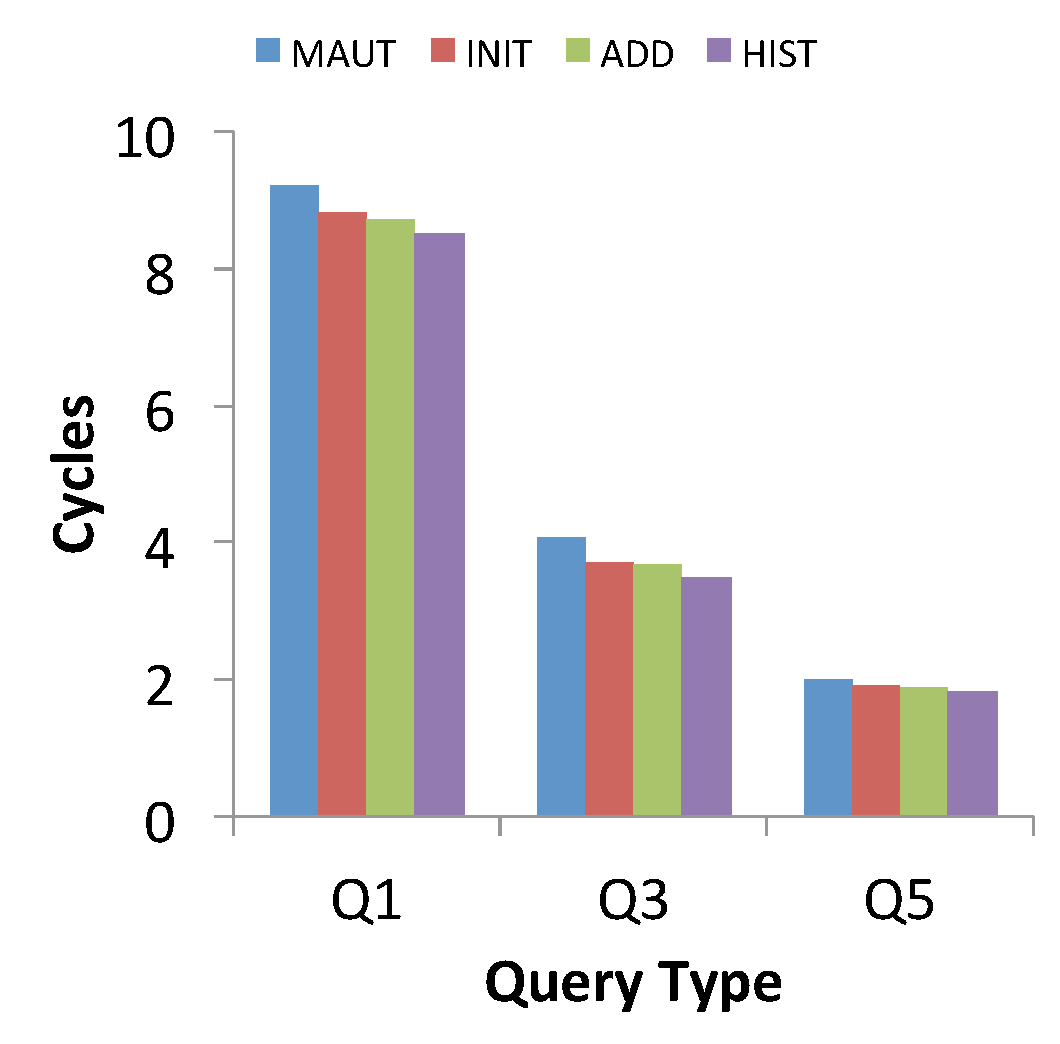
\includegraphics[width=1\linewidth]{figures-bharath/finalMix_camera_opt}
  \caption[]{Average number of interaction cycles on Camera dataset - optimal user model}
  \label{fig:finalMix_camera_opt}
\end{minipage}%
\;\;\;\;\;\;
\begin{minipage}{.45\textwidth}
  \centering
  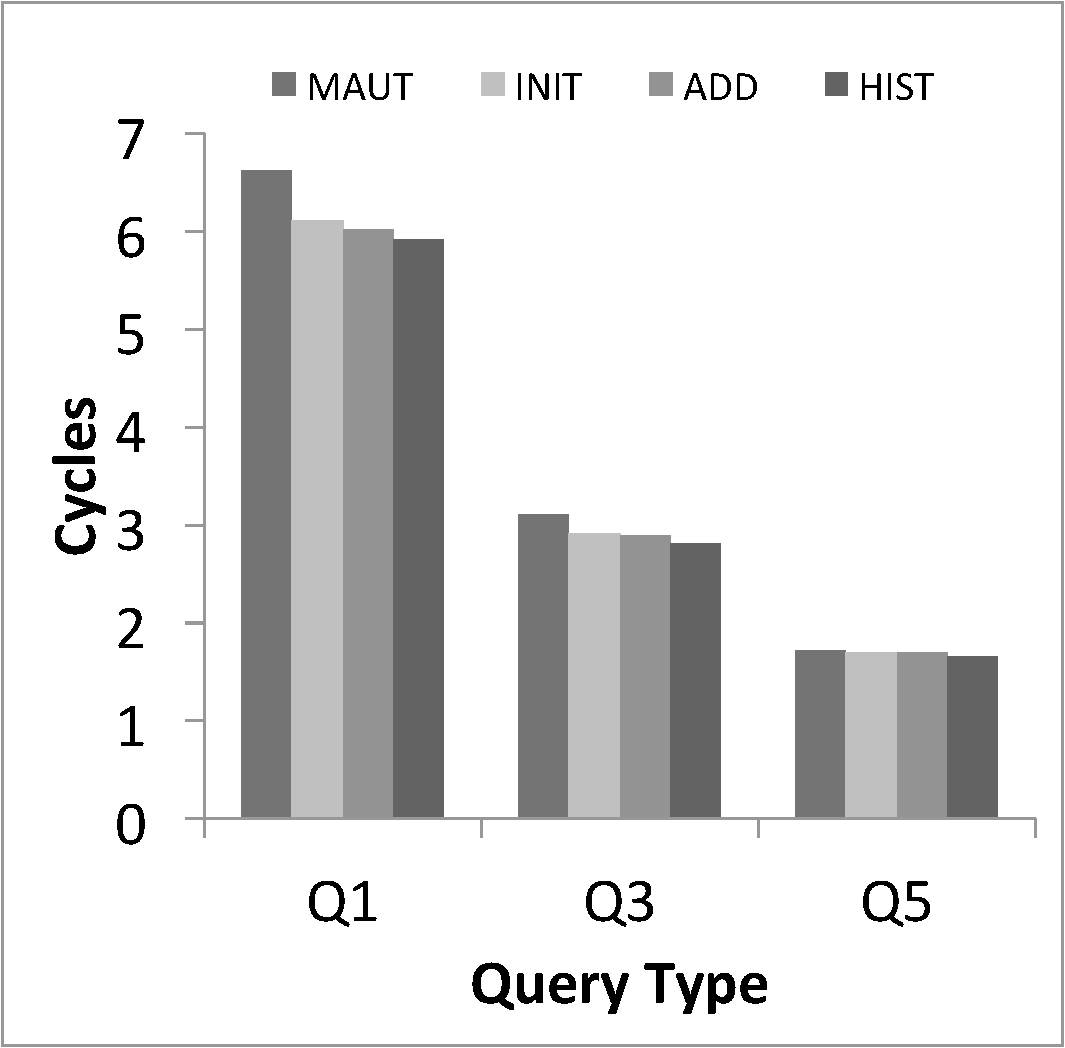
\includegraphics[width=1\linewidth]{figures-bharath/finalMix_pc_opt}
  \caption[]{Average number of interaction cycles on PC dataset - optimal user model}
  \label{fig:finalMix_pc_opt}
\end{minipage}
\end{figure}

\begin{figure}[h]
\centering
\begin{minipage}{.45\textwidth}
  \centering
  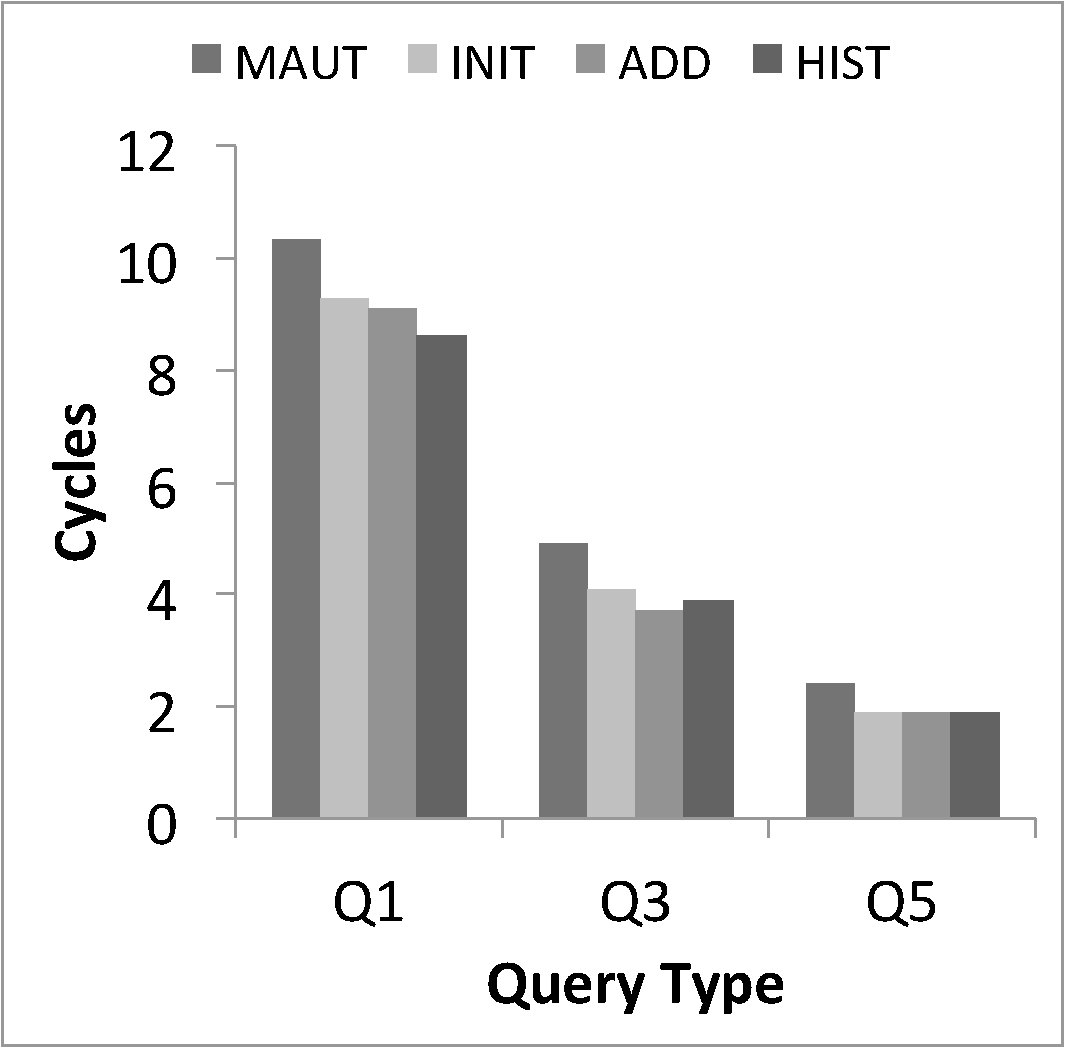
\includegraphics[width=1\linewidth]{figures-bharath/finalMix_camera_noisy}
  \caption[]{Average number of interaction cycles on Camera dataset - noisy framework}
  \label{fig:finalMix_camera_noisy}
\end{minipage}%
\;\;\;\;\;\;
\begin{minipage}{.45\textwidth}
  \centering
  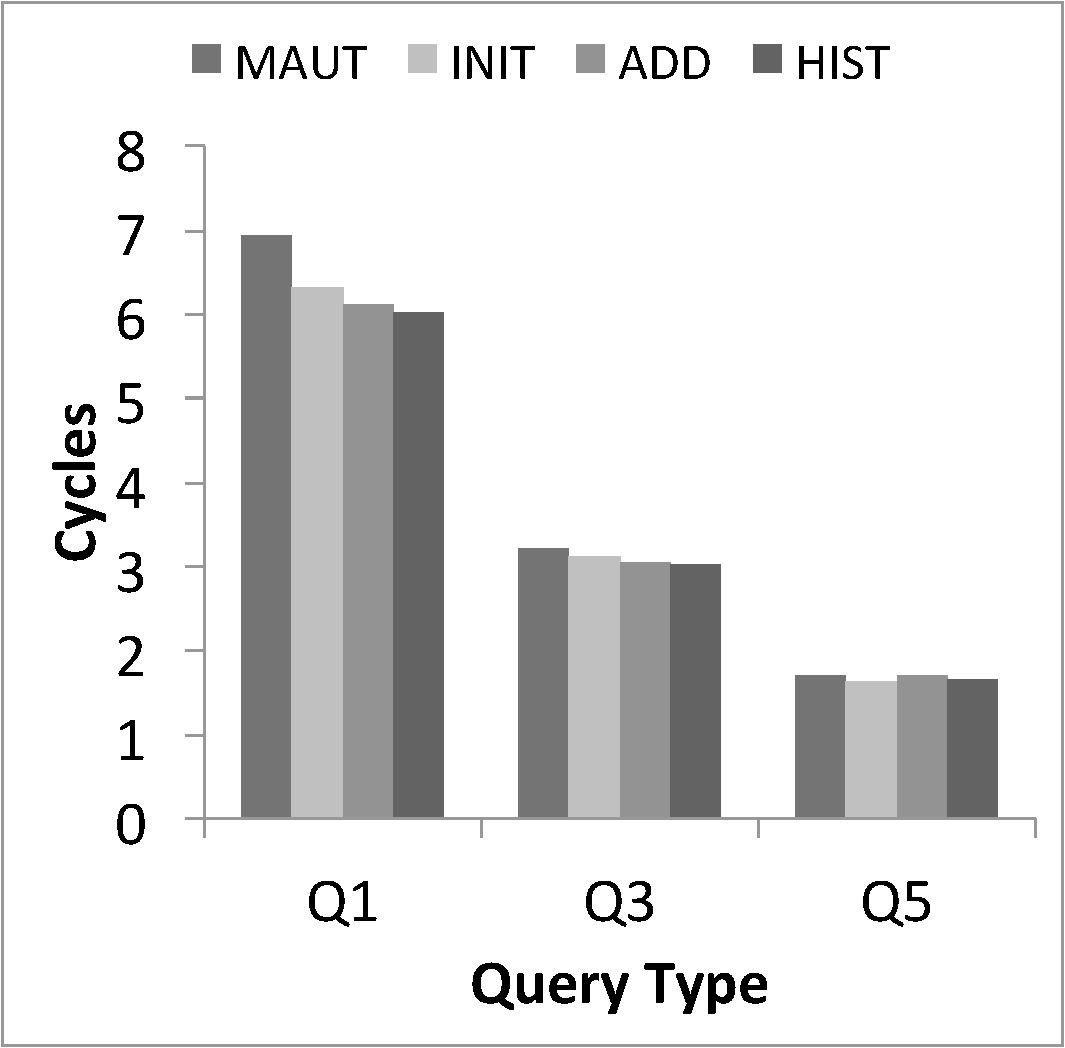
\includegraphics[width=1\linewidth]{figures-bharath/finalMix_pc_noisy}
  \caption[]{Average number of interaction cycles on PC dataset - noisy framework}
  \label{fig:finalMix_pc_noisy}
\end{minipage}
\end{figure}
